\documentclass[tikz, border = 5pt]{standalone}
\usepackage{tikz}

\usetikzlibrary{calc}
\usetikzlibrary{arrows.meta}
\usetikzlibrary{shapes.geometric}

\begin{document}

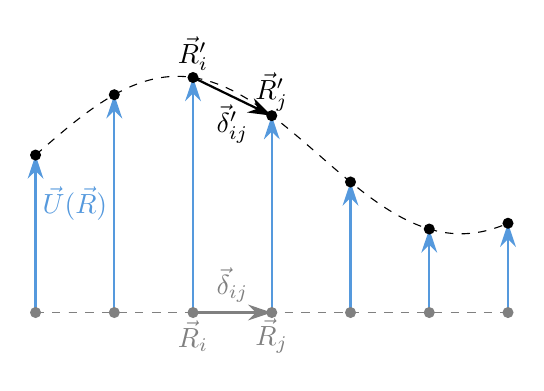
\begin{tikzpicture}[scale = 1.0]

	% model parameters:
	\def \num{7}
	\def \ripos{3}
	\pgfmathtruncatemacro{\rjpos}{\ripos+1}
	\def \verdist{2}
	\def \hordist{1}
	\pgfmathsetmacro{\horend}{\num*\hordist}
	\def \period{50}
	\def \phase{-\period}

	% colors 
	\definecolor{mygrey}{HTML}{808080}
	\definecolor{myblue}{HTML}{5599DD}

	% artistic parameters
	\def \circsize{(2pt)}
	\def \arrcol{myblue}
	\def \arrlw{0.8pt}
	\def \oldcol{mygrey}
	\def \ls {dashed}

	\newcommand{\newpos}[1]{
		\pgfmathsetmacro{\Ynew}{\verdist + sin(#1*\period + \phase)}
	}
	
	% draw contiuous chains
	\draw[\oldcol, domain=\hordist:\horend, \ls, samples = 100] plot (\x, {0});
	\draw[domain=\hordist:\horend, \ls, samples = 100] plot (\x, {\verdist + sin(\x*\period + \phase)});

	% define old and new points
	\foreach \i in {1,...,\num}{
		\pgfmathsetmacro{\X}{\i*\hordist}
		\newpos{\X}

		\coordinate (P-\i-old) at (\X, 0);
		\coordinate (P-\i-new) at (\X, \Ynew);
	}

	% define old and new midpoints between ri and rj
	\coordinate (mid-old) at ($0.5*(P-\ripos-old) + 0.5*(P-\rjpos-old)$);
	\coordinate (mid-new) at ($0.5*(P-\ripos-new) + 0.5*(P-\rjpos-new)$);

	% draw arrows from new to old positions

	\foreach \i in {1,...,\num}{
		\draw[-{Stealth[length=3mm, width=2mm]}, line width = \arrlw, \arrcol] (P-\i-old) -- (P-\i-new);
	}

	% draw old and new NN vectors from Ri to Rj

	\draw[-{Stealth[length=3mm, width=2mm]}, line width = \arrlw, \oldcol] (P-\ripos-old) -- (P-\rjpos-old);
	\draw[-{Stealth[length=3mm, width=2mm]}, line width = \arrlw] (P-\ripos-new) -- (P-\rjpos-new);



	% draw points at old and new positions
	\foreach \i in {1,...,\num}{
		\fill[\oldcol] (P-\i-old) circle \circsize;
		\fill (P-\i-new) circle \circsize;
	}

	% draw new and old position labels

	\node[\oldcol] at (\ripos, -0.3) {$\vec{R}_i$};
	\newpos{\ripos}
	\node at (\ripos, \Ynew + 0.3) {$\vec{R}_i^\prime$};
	\node[\oldcol] at (\rjpos, -0.3) {$\vec{R}_j$};
	\newpos{\rjpos}
	\node at (\rjpos, \Ynew + 0.3) {$\vec{R}_j^\prime$};

	% draw NN vector labels

	\node[\oldcol] at ($(mid-old) + (0, 0.35)$) {$\vec{\delta}_{ij}$};
	\node at ($ (mid-new) + (0, -0.35)$) {$\vec{\delta}_{ij}^\prime$};

	% draw displacement field label

	\coordinate (displace) at ($ 0.5*(P-1-old) + 0.5*(P-2-new) $);
	\node[\arrcol] at (displace) {$\vec{U}(\vec{R})$};

\end{tikzpicture}

\end{document}
